\chapter{Infinite Systems and Symmetry}

% ============================================================
\section{Symmetry and Normal Modes}
% ============================================================

Symmetries of a coupled oscillator system determine the amplitude ratios of its normal modes without ever having to diagonalize the equation of motion. The strategy is: identify a linear transformation $S$ on the configuration space that leaves the equations of motion invariant, then look for normal modes that are simultaneously eigenvectors of $S$.

\begin{definition}[Symmetry matrix]
A \emph{symmetry matrix} $S$ for a coupled oscillator system with configuration vector $\vect{x}(t) = (x_1, x_2, \ldots, x_n)^\top$ is a linear map such that whenever $\vect{x}(t)$ is a solution of the equations of motion, so is $\tilde{\vect{x}}(t) = S\,\vect{x}(t)$. Equivalently, if $K$ is the matrix governing $\ddot{\vect{x}} = -K\vect{x}$ (or $M^{-1}K$ for unequal masses), then $S$ commutes with the dynamical matrix:
\begin{equation}
    SK = KS.
\end{equation}
\end{definition}

\subsection{Reflection Symmetry}

Consider two identical masses connected by three identical springs to two fixed walls, with displacements $x_1$, $x_2$ measured from equilibrium. Reflecting the system about its midpoint swaps the two blocks and negates their displacements: $x_1 \to -x_2$, $x_2 \to -x_1$. The corresponding symmetry matrix is
\begin{equation}
    S = \begin{pmatrix} 0 & -1 \\ -1 & 0 \end{pmatrix}.
\end{equation}

\subsection{Some Common Symmetry Matrices}

\begin{example}[Three blocks in a row]
For three masses $m_1, m_2, m_3$ connected in a chain between two walls with identical springs, several natural symmetry matrices arise:
\begin{align}
    S_{\mathrm{cyc}} &= \begin{pmatrix} 0 & 0 & 1 \\ 1 & 0 & 0 \\ 0 & 1 & 0 \end{pmatrix}
    & &\text{(cyclic shift)}, \\
    S_{\mathrm{ref}} &= \begin{pmatrix} 0 & 0 & -1 \\ 0 & -1 & 0 \\ -1 & 0 & 0 \end{pmatrix}
    & &\text{(reflection)}, \\
    S_{\mathrm{wr}} &= \begin{pmatrix} -1 & 0 & 0 \\ 0 & 0 & -1 \\ 0 & -1 & 0 \end{pmatrix}
    & &\text{(``weird'' reflection: swap two + flip signs)}.
\end{align}
Any solution $\vect{x}(t)$ carried into $S\vect{x}(t)$ by one of these matrices is also a solution.
\end{example}

\subsection{Eigenvalue Equation for Normal Modes}

Suppose $\vect{x}^{(i)}(t) = \vect{A}^{(i)} \cos(\omega_i t + \phi_i)$ is a normal mode with amplitude vector $\vect{A}^{(i)}$ and frequency $\omega_i$. Then $\tilde{\vect{x}} = S \vect{x}^{(i)}$ is also a solution of the equations of motion, and because $S$ is a constant matrix, $\tilde{\vect{x}}$ oscillates at the same frequency $\omega_i$. If all eigenfrequencies are distinct, $\tilde{\vect{x}}$ must therefore be proportional to $\vect{x}^{(i)}$:
\begin{equation}
    \tilde{\vect{x}}(t) = \beta \vect{A}^{(i)} \cos(\omega_i t + \phi_i)
    = S \vect{A}^{(i)} \cos(\omega_i t + \phi_i).
\end{equation}
Stripping off the time dependence gives the central result.

\begin{formula}[Symmetry eigenvalue equation]
Each normal-mode amplitude vector $\vect{A}^{(i)}$ is an eigenvector of every symmetry matrix that commutes with the dynamical matrix:
\begin{equation}
    S \vect{A}^{(i)} = \beta_i\, \vect{A}^{(i)}.
\end{equation}
\end{formula}
This is almost always easier to solve than the full matrix equation $M^{-1}K\vect{A} = \omega^2 \vect{A}$, since $S$ typically has small integer entries and a trivial characteristic polynomial. The one caveat is that the argument requires the eigenfrequencies to be nondegenerate; if two modes share a frequency, any linear combination of them is also a normal mode at that frequency, and the eigenvectors of $S$ must then be chosen carefully within the degenerate subspace.

\subsection{Example: Two-Mass Reflection}

For the two-mass reflection system with $S = \begin{pmatrix} 0 & -1 \\ -1 & 0 \end{pmatrix}$, the eigenvalue equation $(S - \beta I)\vect{A} = 0$ requires
\begin{equation}
    \det\begin{pmatrix} -\beta & -1 \\ -1 & -\beta \end{pmatrix} = \beta^2 - 1 = 0 \implies \beta = \pm 1.
\end{equation}
For $\beta = +1$: $-A_2 = A_1 \implies A_2 = -A_1$ (antisymmetric mode). For $\beta = -1$: $-A_2 = -A_1 \implies A_2 = A_1$ (symmetric mode). The amplitude ratios drop out immediately, without ever writing down the equations of motion.

\begin{fact}
The eigenvalues $\beta$ of a symmetry matrix $S$ representing a discrete geometric operation (reflection, cyclic shift, \ldots) satisfy $|\beta| = 1$. Otherwise repeated application of $S$ would blow up or shrink the amplitudes without bound.
\end{fact}

% ============================================================
\section{Infinite Chain of Oscillators}
% ============================================================

We now take the ideas of the previous section to their natural extreme. Instead of two or three coupled blocks, consider an infinite chain of identical masses $m$ connected by identical springs of constant $k$ and equilibrium separation $a$, as in Figure~\ref{fig:spring-chain}. Let $x_j(t)$ denote the (longitudinal) displacement of block $j$ from its equilibrium position. The chain has infinitely many degrees of freedom, but it also has an exact discrete translational symmetry, and that single fact will be enough to solve it completely.

\begin{figure}[H]
    \centering
    \begin{tikzpicture}[>=Stealth, every node/.style={font=\small}]
        \tikzset{spring/.style={decorate, decoration={coil, aspect=0.6, segment length=4pt, amplitude=4.5pt, pre length=5pt, post length=5pt}}}
        \def\a{2.4}
        % equilibrium reference lines for the labelled masses
        \foreach \i in {1,2,3} {
            \draw[gray!55, dashed] ({\a*\i},-0.75) -- ({\a*\i},1.2);
        }
        % masses, some displaced from equilibrium
        \foreach \i/\dx in {0/0, 1/0.34, 2/-0.26, 3/0.38, 4/0} {
            \node[draw, fill=LightGray, minimum size=0.6cm, inner sep=0] (m\i) at ({\a*\i+\dx},0) {};
        }
        % springs
        \draw[spring] ({-\a*0.6},0) -- (m0.west);
        \draw[spring] (m0.east) -- (m1.west);
        \draw[spring] (m1.east) -- (m2.west);
        \draw[spring] (m2.east) -- (m3.west);
        \draw[spring] (m3.east) -- (m4.west);
        \draw[spring] (m4.east) -- ({\a*4+\a*0.6},0);
        % index labels
        \foreach \i/\lab in {1/{j-1}, 2/{j}, 3/{j+1}} {
            \node[below=3pt] at (m\i.south) {$\lab$};
        }
        % displacement arrows measured from the dashed equilibrium lines
        \foreach \i/\dx/\lab in {1/0.34/{x_{j-1}}, 2/-0.26/{x_j}, 3/0.38/{x_{j+1}}} {
            \draw[->, thick] ({\a*\i},0.78) -- ({\a*\i+\dx},0.78);
            \node[above] at ({\a*\i+\dx/2},0.82) {$\lab$};
        }
        \node at ({-\a*0.9},0) {$\cdots$};
        \node at ({\a*4+\a*0.9},0) {$\cdots$};
    \end{tikzpicture}
    \caption{An infinite chain of identical masses $m$ joined by identical springs of stiffness $k$ and equilibrium spacing $a$. Dashed lines mark the equilibrium positions; arrows indicate the instantaneous displacements $x_j$ of the individual blocks.}
    \label{fig:spring-chain}
\end{figure}

Newton's second law for block $j$ reads
\begin{equation}
    m\ddot{x}_j = -k(x_j - x_{j-1}) + k(x_{j+1} - x_j) = k\,(x_{j-1} - 2 x_j + x_{j+1}).
\end{equation}
Defining $\omega_0^2 \defeq k/m$, the equation of motion becomes
\begin{equation}
    \ddot{x}_j = \omega_0^2 \,(x_{j-1} - 2 x_j + x_{j+1}).
\end{equation}

\subsection{Ansatz and Dispersion Relation}

Try a normal-mode ansatz with common frequency $\omega$,
\begin{equation}
    x_j(t) = A_j\, e^{i\omega t}, \qquad \ddot{x}_j = -\omega^2 A_j\, e^{i\omega t}.
\end{equation}
Substituting and cancelling $e^{i\omega t}$,
\begin{equation}
    \omega^2 A_j = \omega_0^2\,(-A_{j-1} + 2 A_j - A_{j+1}).
\end{equation}

\subsection{Translational Symmetry}

The infinite chain has a discrete translational symmetry: shifting every block one lattice site is a symmetry of the equations of motion. The relationship between blocks $j$ and $j+1$ must equal the relationship between blocks $j+1$ and $j+2$. Concretely, the symmetry matrix $S$ shifts the amplitude vector $\vect{A} = (\ldots, A_{j-1}, A_j, A_{j+1}, \ldots)^\top$ up by one entry, so that $S\vect{A}$ has components $A_{j+1}$ at position $j$:
\begin{equation}
    S = \begin{pmatrix}
        \ddots & \ddots & & & \\
         & 0 & 1 & & \\
         & & 0 & 1 & \\
         & & & 0 & 1 \\
         & & & & \ddots
    \end{pmatrix}.
\end{equation}
By the eigenvalue equation $S\vect{A} = \beta \vect{A}$, adjacent amplitudes must be related by a constant ratio:
\begin{equation}
    A_{j+1} = \beta A_j \iff A_j = \beta^j A_0.
\end{equation}
Substituting into the recursion,
\begin{equation}
    \omega^2 = \omega_0^2 \left(-\frac{A_{j-1}}{A_j} + 2 - \frac{A_{j+1}}{A_j}\right) = \omega_0^2\!\left(-\frac{1}{\beta} + 2 - \beta\right).
\end{equation}
For the solution not to blow up as $|j| \to \infty$ we require $|\beta| = 1$, so we set
\begin{equation}
    \beta \defeq e^{ika},
\end{equation}
where $k$ is a real parameter with units of inverse length, the \emph{wavenumber}, and $a$ is the equilibrium separation. Then $1/\beta + \beta = 2\cos(ka)$, and

\begin{formula}[Dispersion relation for the beaded spring chain]
\begin{equation}
    \omega^2 = 2\omega_0^2 \bigl(1 - \cos(ka)\bigr).
\end{equation}
\end{formula}
Using the half-angle identity $1 - \cos(ka) = 2\sin^2(ka/2)$, this takes the equivalent and often more useful form
\begin{equation}
    \omega = 2\omega_0\,\left|\sin\!\left(\tfrac{ka}{2}\right)\right|,
\end{equation}
plotted in Figure~\ref{fig:monatomic-dispersion}. A \emph{dispersion relation} is any such functional relationship $\omega(k)$ between frequency and wavenumber; it encodes everything about how the medium propagates waves. Two features stand out. First, $\omega$ is periodic in $k$ with period $2\pi/a$, so wavenumbers differing by a reciprocal-lattice step $2\pi/a$ describe the very same motion of the discrete blocks; it suffices to keep $k$ in the interval $(-\pi/a, \pi/a]$, the \emph{first Brillouin zone}. Second, the curve flattens as $k \to \pm\pi/a$, where $\omega$ saturates at its maximum value $2\omega_0$.

\begin{figure}[H]
    \centering
    \begin{tikzpicture}
    \begin{axis}[
        width=0.82\textwidth, height=0.46\textwidth,
        xlabel={$k$}, ylabel={$\omega$},
        xmin=-3.55, xmax=3.55, ymin=0, ymax=2.35,
        xtick={-3.14159,-1.5708,0,1.5708,3.14159},
        xticklabels={$-\pi/a$,$-\pi/2a$,$0$,$\pi/2a$,$\pi/a$},
        ytick={1,2}, yticklabels={$\omega_0$,$2\omega_0$},
        axis lines=left,
        samples=200, domain=-3.14159:3.14159,
        clip=false,
    ]
    \draw[gray, dashed] (axis cs:-3.14159,2) -- (axis cs:3.14159,2);
    \draw[gray!60, dashed] (axis cs:-3.14159,0) -- (axis cs:-3.14159,2);
    \draw[gray!60, dashed] (axis cs:3.14159,0) -- (axis cs:3.14159,2);
    \addplot[blue, thick, smooth] {2*abs(sin(deg(x/2)))};
    \end{axis}
    \end{tikzpicture}
    \caption{The dispersion relation $\omega = 2\omega_0\,|\sin(ka/2)|$ for the monatomic chain, shown across the first Brillouin zone $-\pi/a < k \le \pi/a$. The frequency rises linearly from the origin (nondispersive, sound-like behaviour) and saturates at the cutoff $2\omega_0$ at the zone boundary $k = \pm\pi/a$.}
    \label{fig:monatomic-dispersion}
\end{figure}

\subsection{Spatial Form of the Modes}

Since $A_j = \beta^j A_0 = e^{ikja} A_0$ and $x = j a$ is the equilibrium position of block $j$ along the chain, the amplitude sampled on the lattice is
\begin{equation}
    A_j \propto e^{ikja} = e^{ikx}.
\end{equation}
An equally valid choice is $\beta = e^{-ika}$, giving $A_j \propto e^{-ikx}$. Real linear combinations of the two produce the standing-wave form
\begin{equation}
    x_j(t) = C \cos(k j a + \alpha)\, e^{i\omega t},
\end{equation}
or, taking the real part,
\begin{equation}
    x_j(t) = C \cos(k j a + \alpha) \cos(\omega t + \phi),
\end{equation}
with $\omega^2 = 2\omega_0^2(1 - \cos(ka))$.

\begin{fact}[Bandwidth of the chain]
Because $\cos(ka)$ ranges over $[-1, 1]$, only frequencies with
\begin{equation}
    0 \leq \omega \leq 2\omega_0
\end{equation}
propagate on the chain, as Figure~\ref{fig:monatomic-dispersion} makes plain. All others are forbidden: the finite lattice spacing imposes a cutoff, a feature with no analogue in the continuous string.
\end{fact}

The infinitely many $(k, \omega)$ pairs are all normal modes; any solution is a linear combination
\begin{equation}
    x_j(t) = \sum_i C_i \cos(k_i\, j a + \alpha_i) \cos(\omega_i t + \phi_i).
\end{equation}

\begin{formula}[Wavelength]
The wavenumber $k$ and wavelength $\lambda$ are related by
\begin{equation}
    \lambda = \frac{2\pi}{k}.
\end{equation}
\end{formula}

\subsection{Symmetry and Commutators}

The pattern behind all of this is that if $S$ is a symmetry of the equations of motion $\ddot{\vect{x}} = -K \vect{x}$, then $S$ commutes with $K$:
\begin{equation}
    SK = KS.
\end{equation}
Two commuting matrices share a common eigenbasis, so simultaneously diagonalizing $K$ and $S$ gives normal modes labeled by both a frequency $\omega$ and a symmetry eigenvalue $\beta$.

If $\vect{A}$ and $\vect{A}'$ are two normal modes of the system with the \emph{same} angular frequency, then any linear combination $b\vect{A} + c\vect{A}'$ is also a normal mode at that frequency. This is the loophole in the symmetry-eigenvector argument.

% ============================================================
\section{Boundary Conditions on Finite Chains}
% ============================================================

The infinite chain is an idealization; real systems are finite. Rather than redo the whole normal-mode analysis with a truncated dynamical matrix, we exploit the work already done: embed the finite chain inside a fictitious infinite one, and impose \emph{boundary conditions} whose only role is to pick out the finite subset of modes that are physically realized. In this way the machinery of translational symmetry survives even when translational symmetry itself is broken by the endpoints.

\subsection{Fixed Wall on the Left}

Consider $n$ masses connected by identical springs, with the leftmost spring attached to a wall at $j = 0$. Model this by treating the wall as a fictitious block ``$0$'' at $j = 0$ that never moves: $x_0(t) = 0$ for all $t$. Using the general infinite-chain solution
\begin{equation}
    x_j(t) = C\cos(k j a + \alpha) \cos(\omega t + \phi),
\end{equation}
the condition $x_0 = 0$ gives $\cos(\alpha) = 0$, so $\alpha = \pi/2$. Then
\begin{equation}
    x_j(t) = C\sin(k j a)\cos(\omega t + \phi).
\end{equation}

\subsection{Fixed Wall on the Right}

If a second wall sits at position $j = n+1$, then $x_{n+1}(t) = 0$ requires $\sin\bigl(k(n+1)a\bigr) = 0$, i.e.\
\begin{equation}
    k(n+1)a = m\pi, \qquad m \in \mathbb{Z}.
\end{equation}
Hence

\begin{formula}[Quantized wavenumbers, wall--wall boundary conditions]
\begin{equation}
    k_m = \frac{m\pi}{(n+1)a}, \qquad \lambda_m = \frac{2(n+1)a}{m},
\end{equation}
for $m = 1, 2, \ldots, n$.
\end{formula}
Distinct choices of $m$ give the $n$ physically distinct normal modes:
\begin{equation}
    x_j^{(m)}(t) = C_m \sin\!\left(\frac{m\pi\, j}{n+1}\right) \cos(\omega_m t + \phi_m),
\end{equation}
where each $\omega_m$ is determined by the dispersion relation
\begin{equation}
    \omega_m = \sqrt{2\omega_0^2\bigl(1 - \cos(k_m a)\bigr)}.
\end{equation}
The remaining $2n$ free parameters --- $C_m$ and $\phi_m$ for each of the $n$ modes --- are fixed by the $2n$ initial conditions (position and velocity of each block).

\begin{example}[Five beads on a string, fixed ends]
A string of tension $T$ is pinned to walls at $x = 0$ and $x = 6a$, with five identical beads of mass $m$ threaded on it at $x = a, 2a, \ldots, 5a$. Find the normal-mode frequencies.

Because both ends are pinned, the earlier analysis with $n = 5$ applies: the allowed wavenumbers are $k_m a = m\pi/6$ for $m = 1, 2, 3, 4, 5$. Substituting into the dispersion relation $\omega_m^2 = 2\omega_0^2\bigl(1 - \cos(k_m a)\bigr)$ with $\omega_0^2 = T/(ma)$, and using the half-angle identity $1 - \cos\theta = 2\sin^2(\theta/2)$,
\begin{equation}
    \omega_m = 2\omega_0 \sin\!\left(\frac{m\pi}{12}\right), \qquad m = 1, \ldots, 5.
\end{equation}
The lowest mode $m = 1$ has the whole string bowing in a single arch; the top mode $m = 5$ has adjacent beads nearly out of phase (Figure~\ref{fig:mode-shapes}). Notice $\omega_5 = 2\omega_0 \sin(5\pi/12) < 2\omega_0$: the discrete lattice never quite saturates the cutoff bandwidth because $k = \pi/a$ is not in the allowed set.
\end{example}

\begin{figure}[H]
    \centering
    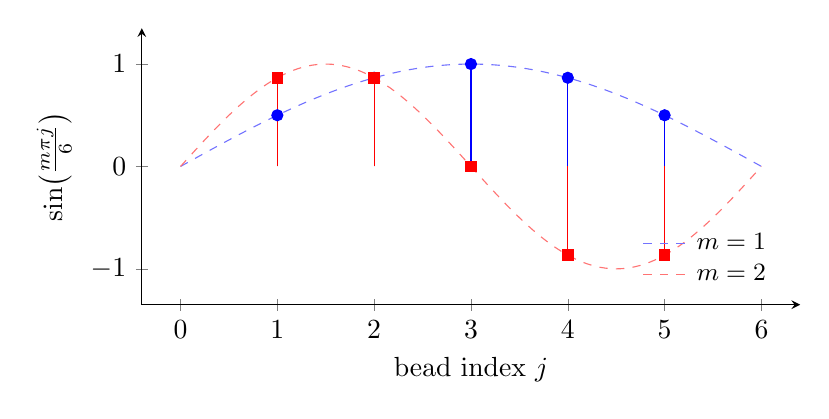
\begin{tikzpicture}
    \begin{axis}[
        width=0.82\textwidth, height=0.42\textwidth,
        xlabel={bead index $j$},
        ylabel={$\sin\!\left(\frac{m\pi j}{6}\right)$},
        xmin=-0.4, xmax=6.4, ymin=-1.35, ymax=1.35,
        xtick={0,1,2,3,4,5,6},
        ytick={-1,0,1},
        axis lines=left,
        legend pos=south east,
        legend style={font=\small, draw=none, fill=none},
        clip=false,
    ]
    % continuous envelopes
    \addplot[blue!55, dashed, domain=0:6, samples=100] {sin(deg(pi*x/6))};
    \addplot[red!55, dashed, domain=0:6, samples=120] {sin(deg(2*pi*x/6))};
    % stems m=1
    \addplot[blue, only marks, mark=*, mark size=2pt] coordinates {(1,0.5)(2,0.866)(3,1)(4,0.866)(5,0.5)};
    \addplot[blue, ycomb] coordinates {(1,0.5)(2,0.866)(3,1)(4,0.866)(5,0.5)};
    % stems m=2
    \addplot[red, only marks, mark=square*, mark size=1.9pt] coordinates {(1,0.866)(2,0.866)(3,0)(4,-0.866)(5,-0.866)};
    \addplot[red, ycomb] coordinates {(1,0.866)(2,0.866)(3,0)(4,-0.866)(5,-0.866)};
    \legend{$m=1$,$m=2$}
    \end{axis}
    \end{tikzpicture}
    \caption{Spatial profiles of the $m = 1$ and $m = 2$ normal modes of five beads with both ends fixed ($n = 5$). Markers give the bead amplitudes $\propto \sin(m\pi j/6)$; dashed curves are the continuous standing-wave envelopes they sample. The fictitious wall blocks at $j = 0$ and $j = 6$ sit at nodes.}
    \label{fig:mode-shapes}
\end{figure}

% ============================================================
\section{Beads on a String}
% ============================================================

The beaded spring chain assumes longitudinal motion against restoring springs, but the same mathematics arises whenever the restoring force is linear in nearest-neighbor differences. The classic transverse analogue is a row of beads on a stretched string, shown in Figure~\ref{fig:beads-string}: $n$ identical beads of mass $m$ are threaded onto a massless string held at tension $T$, with equilibrium separation $a$. The beads move only transversely, with small displacements $y_j$ in the $y$-direction. As we will see, the tension supplies exactly the linear restoring force that the springs did before, so the entire analysis carries over unchanged.

\begin{figure}[H]
    \centering
    \begin{tikzpicture}[>=Stealth, every node/.style={font=\small}]
        \def\a{1.7}
        % walls
        \draw[thick] (0,-0.7) -- (0,0.95);
        \draw[thick] ({6*\a},-0.7) -- ({6*\a},0.95);
        \foreach \yw in {-0.6,-0.4,...,0.85} {
            \draw[gray] (-0.16,{\yw}) -- (0,{\yw+0.16});
            \draw[gray] ({6*\a},{\yw+0.16}) -- ({6*\a+0.16},{\yw});
        }
        % equilibrium line
        \draw[gray!55, dashed] (0,0) -- ({6*\a},0);
        % bead positions (transverse displacements)
        \coordinate (b0) at (0,0);
        \coordinate (b1) at ({1*\a},0.42);
        \coordinate (b2) at ({2*\a},0.66);
        \coordinate (b3) at ({3*\a},0.34);
        \coordinate (b4) at ({4*\a},-0.30);
        \coordinate (b5) at ({5*\a},-0.14);
        \coordinate (b6) at ({6*\a},0);
        % string
        \draw[thick] (b0)--(b1)--(b2)--(b3)--(b4)--(b5)--(b6);
        % beads
        \foreach \i in {1,...,5} { \fill[blue!70!black] (b\i) circle (2.6pt); }
        % displacement arrow for one bead
        \draw[->, thick] ({2*\a},0) -- (b2);
        \node[right] at ({2*\a+0.05},0.36) {$y_j$};
        % spacing marker a
        \draw[<->] (0,-0.55) -- ({1*\a},-0.55);
        \node[below] at ({0.5*\a},-0.55) {$a$};
    \end{tikzpicture}
    \caption{Beads of mass $m$ on a string of tension $T$, fixed at both walls. Each bead is displaced transversely by a small amount $y_j$; the tension in the tilted string segments provides the restoring force.}
    \label{fig:beads-string}
\end{figure}

\subsection{Equation of Motion}

Consider bead $j$ with left and right neighbors at $y_{j-1}$ and $y_{j+1}$. The string pulls the bead in both directions with tension $T$; the vertical components of these forces are $-T\sin\theta_1$ (from the left) and $-T\sin\theta_2$ (from the right). In the small-angle approximation $\sin\theta \approx \tan\theta$, we have
\begin{equation}
    \sin\theta_1 \approx \frac{y_j - y_{j-1}}{a}, \qquad \sin\theta_2 \approx \frac{y_j - y_{j+1}}{a}.
\end{equation}
(Gravity is dropped as it merely shifts the equilibrium.) Newton's law gives
\begin{equation}
    m\ddot{y}_j = -T\,\frac{y_j - y_{j-1}}{a} - T\,\frac{y_j - y_{j+1}}{a} = \frac{T}{a}\,(y_{j-1} - 2 y_j + y_{j+1}).
\end{equation}
Hence

\begin{formula}[Beaded-string EOM]
\begin{equation}
    \ddot{y}_j = \frac{T}{ma}\,(y_{j-1} - 2 y_j + y_{j+1}).
\end{equation}
\end{formula}

\subsection{Dispersion Relation}

Guess $y_j(t) = A_j e^{i\omega t}$ so that $\ddot{y}_j = -\omega^2 A_j e^{i\omega t}$. Substituting,
\begin{equation}
    -\omega^2 A_j = \frac{T}{ma}\,(A_{j-1} - 2 A_j + A_{j+1}).
\end{equation}
Translational symmetry again dictates $A_{j+1} = \beta A_j$ with $\beta = e^{ika}$. Defining $\omega_0^2 \defeq T/(ma)$,
\begin{equation}
    \omega^2 = \omega_0^2\!\left(2 - e^{-ika} - e^{ika}\right)
    = 2\omega_0^2 \bigl(1 - \cos(ka)\bigr),
\end{equation}
identical in form to the beaded spring chain. Consequently the normal modes are again
\begin{equation}
    y_j^{(m)}(t) = C\cos(k j a + \alpha)\cos(\omega t + \phi).
\end{equation}

\subsection{Massless-Ring (Free-End) Boundary Conditions}

Suppose the string ends at massless frictionless rings that can slide freely in the transverse direction. Since the ring is massless, the transverse net force on it must vanish (else infinite acceleration). On the left end, the vertical component of the tension from the string segment connecting rings $0$ and $1$ gives
\begin{equation}
    0 = -T \sin\theta \approx -T\,\frac{y_0 - y_1}{a} \implies y_0 = y_1.
\end{equation}
Similarly the right end gives $y_n = y_{n+1}$.

\subsection{Complex-Exponential Solution and Quantization}

Instead of using the sinusoidal form, write the general solution as a sum of the two allowed complex exponentials at wavenumber $k$:
\begin{equation}
    y_j(t) = \bigl(A e^{ikja} + B e^{-ikja}\bigr)\cos(\omega t + \phi).
\end{equation}
Impose $y_0 = y_1$:
\begin{equation}
    A + B = A e^{ika} + B e^{-ika}
    \implies A(1 - e^{ika}) = B(e^{-ika} - 1). \tag{$\ast$}
\end{equation}
Impose $y_n = y_{n+1}$:
\begin{equation}
    A e^{ikna}(1 - e^{ika}) = B e^{-ikna}(e^{-ika} - 1). \tag{$\ast\ast$}
\end{equation}
Dividing $(\ast\ast)$ by $(\ast)$ gives $e^{ikna} = e^{-ikna}$, so $2 k n a = 2\pi m$, i.e.\

\begin{formula}[Quantized wavenumbers, free--free boundary conditions]
\begin{equation}
    k_m = \frac{m\pi}{n a}, \qquad m \in \mathbb{Z}.
\end{equation}
\end{formula}
Back-substituting into $(\ast)$ shows $B = A e^{ika}$, so
\begin{equation}
    y_j(t) = A\,\bigl(e^{i j k a} + e^{-i(j-1)ka}\bigr)\cos(\omega t + \phi),
\end{equation}
with $\omega_m = \omega_0 \sqrt{2\bigl(1 - \cos(k_m a)\bigr)}$.

\subsection{Mixed Boundary Conditions}

If the left end is a free ring and the right end is fixed to a wall a distance $a/2$ past the last bead, the conditions become
\begin{equation}
    y_0 = y_1, \qquad y_n = -y_{n+1},
\end{equation}
where the second follows from reflecting the ``ghost'' bead through the wall. Analogous quantization conditions on $k$ result, shifted by half-integer amounts relative to the pure fixed-wall or pure free-ring cases.

\begin{example}[Mixed boundary quantization]
For $n$ beads with a free ring at the left ($y_0 = y_1$) and a fixed wall a half-spacing past the last bead ($y_n = -y_{n+1}$), we can seek the sinusoidal form $y_j = C\cos(kja + \alpha)\cos(\omega t + \phi)$. The left condition $\cos(\alpha) = \cos(ka + \alpha)$ is solved by $\alpha = -ka/2$, so that the cosine profile is symmetric about $j = 1/2$ --- geometrically, the free ring sits at an antinode. The right condition $\cos(kna - ka/2) = -\cos(k(n+1)a - ka/2)$ then forces
\begin{equation}
    k_m\,\bigl(n + \tfrac{1}{2}\bigr) a = \bigl(m - \tfrac{1}{2}\bigr)\pi, \qquad m = 1, 2, \ldots, n,
\end{equation}
i.e.\ $k_m a$ is displaced by exactly a quarter-wavelength relative to the wall--wall spectrum. The corresponding frequencies follow from the same dispersion relation.
\end{example}

% ============================================================
\section{The Continuum Limit and the Wave Equation}
% ============================================================

So far every system has been discrete: countably many degrees of freedom, one per bead. To make contact with continuum physics --- vibrating strings, sound waves, light --- we take the beaded string and let the masses become very small and very densely packed, keeping the linear mass density fixed. The discrete recursion collapses onto a second spatial derivative, and we recover a continuous string obeying the wave equation.

\subsection{Continuum Limit}

Re-index the beads by their equilibrium position $x = ja$ along the string, so $y_j(t) \to y(x, t)$. The discrete EOM
\begin{equation}
    \ddot{y}(x,t) = \frac{T}{ma}\,\bigl(y(x-a, t) - 2 y(x,t) + y(x+a, t)\bigr)
\end{equation}
suggests introducing the linear mass density
\begin{equation}
    \rho_L \defeq \frac{m}{a}, \qquad [\rho_L] = \frac{\text{mass}}{\text{length}},
\end{equation}
so that $ma = \rho_L a^2$ and
\begin{equation}
    \ddot{y}(x,t) = \frac{T}{\rho_L a^2}\,\bigl(y(x-a, t) - 2 y(x,t) + y(x+a,t)\bigr).
\end{equation}
Now let $a \to 0$ and $m \to 0$ together, keeping $\rho_L$ fixed. Taylor-expand:
\begin{equation}
    y(x \pm a, t) \approx y(x,t) \pm a\, y'(x,t) + \tfrac{1}{2} a^2 y''(x,t) + \cdots.
\end{equation}
The first-derivative terms cancel, leaving
\begin{equation}
    y(x-a,t) - 2 y(x,t) + y(x+a,t) \approx a^2 y''(x,t).
\end{equation}
Substituting,
\begin{equation}
    \ddot{y}(x,t) = \frac{T}{\rho_L}\, y''(x,t).
\end{equation}

\begin{formula}[Wave equation for a continuous string]
\begin{equation}
    \pdv[2]{y}{t} = \frac{T}{\rho_L}\, \pdv[2]{y}{x}.
\end{equation}
\end{formula}
This is one of the most important equations in all of physics, describing not only strings but sound, light, and any small-amplitude propagating disturbance in a linear medium.

\subsection{Continuum Dispersion Relation}

Taking the same continuum limit inside the discrete dispersion relation, $\cos(ka) \approx 1 - \tfrac{1}{2}(ka)^2$ for $ka \to 0$, so
\begin{equation}
    \omega^2 = 2\omega_0^2\bigl(1 - \cos(ka)\bigr) \approx \omega_0^2 k^2 a^2 = \frac{T}{\rho_L}\, k^2.
\end{equation}
Hence

\begin{formula}[Continuum dispersion relation]
\begin{equation}
    \omega = \sqrt{\frac{T}{\rho_L}}\, k \equiv v_p\, k,
\end{equation}
where $v_p = \sqrt{T/\rho_L}$ is the phase velocity.
\end{formula}
This is a \emph{linear} dispersion relation --- the wave is nondispersive, in contrast with the full lattice which distorts wave packets at wavelengths comparable to $a$.

% ============================================================
\section{General Wave Equation by Separation of Variables}
% ============================================================

More generally, consider
\begin{equation}
    \pdv[2]{\psi}{t} = v_p^2\, \pdv[2]{\psi}{x}.
\end{equation}
Look for separable solutions $\psi(x,t) = A(x) B(t)$. Substituting,
\begin{equation}
    A(x) \ddot{B}(t) = v_p^2\, B(t) A''(x)
    \implies \frac{1}{v_p^2}\frac{\ddot{B}(t)}{B(t)} = \frac{A''(x)}{A(x)}.
\end{equation}
The left side depends only on $t$, the right only on $x$; both must equal a common constant, call it $-k_m^2$. This yields two independent ODEs:
\begin{align}
    \ddot{B}(t) &= -k_m^2 v_p^2\, B(t) \implies B(t) = B_m \sin(\omega_m t + \beta_m),\\
    A''(x) &= -k_m^2 A(x) \implies A(x) = A_m \sin(k_m x + \alpha_m),
\end{align}
with $\omega_m = v_p k_m$.

\begin{formula}[$m$-th normal mode of the continuous string]
\begin{equation}
    \psi_m(x,t) = A_m \sin(k_m x + \alpha_m)\, \sin(\omega_m t + \beta_m).
\end{equation}
\end{formula}
The general solution is a superposition
\begin{equation}
    \psi(x,t) = \sum_m A_m \sin(k_m x + \alpha_m)\, \sin(\omega_m t + \beta_m).
\end{equation}
The unknowns split cleanly according to what fixes them. The relation between $\omega_m$ and $k_m$ is the dispersion relation, which is a statement about the medium itself (its tension, density, and lattice structure). The phase $\alpha_m$ together with the discrete set of allowed $k_m$ is fixed by the spatial boundary conditions, since those are what select which standing-wave shapes fit in the given interval. Finally, the amplitude $A_m$ and temporal phase $\beta_m$ of each mode are fixed by the initial conditions --- the displacement and velocity profiles at $t = 0$.

\subsection{Fixed-End Boundary Conditions}

A string of length $L$ pinned at both ends, $\psi(0, t) = \psi(L, t) = 0$, forces
\begin{equation}
    \sin(\alpha_m) = 0 \implies \alpha_m = 0,
\end{equation}
and
\begin{equation}
    \sin(k_m L) = 0 \implies k_m L = m\pi, \qquad m = 1, 2, 3, \ldots.
\end{equation}
Hence

\begin{formula}[Quantized wavenumbers on a pinned string]
\begin{equation}
    k_m = \frac{m\pi}{L}, \qquad \omega_m = v_p k_m = \frac{m\pi v_p}{L}.
\end{equation}
\end{formula}
The full mode is
\begin{equation}
    \psi_m(x,t) = A_m \sin\!\left(\frac{m\pi x}{L}\right)\sin(\omega_m t + \beta_m),
\end{equation}
identical in form to the finite-bead result of the previous section, with $L = (n+1) a$ in the many-bead limit.

% ============================================================
\section{Diatomic Chain: Acoustic and Optical Branches}
% ============================================================

Every system so far has been perfectly uniform, with one mass per lattice site. The richest new physics of discrete lattices appears the instant we break that uniformity, and the simplest way to do so is to alternate two different masses along the chain. This turns out to be the microscopic origin of why ionic crystals reflect infrared light, so it is worth working through.

Consider a chain with alternating masses $m_1$ and $m_2$ connected by springs of constant $T/a$ (or equivalently a beaded string with alternating bead masses). The equilibrium spacing between neighbours is still $a$, but the repeating unit --- the \emph{unit cell} --- now contains two beads and has length $2a$. Index the two sublattices by even and odd $j$: label the mass at position $2j$ by $m_1$ and at position $2j+1$ by $m_2$.

The translational symmetry now shifts by \emph{two} lattice sites, so use two ansatze:
\begin{equation}
    y_{2j}(t) = A\, e^{i k a (2j)}\, e^{i\omega^{(k)} t},
    \qquad
    y_{2j+1}(t) = B\, e^{i k a (2j+1)}\, e^{i\omega^{(k)} t}.
\end{equation}
Substituting into the equations of motion for each sublattice and cancelling common phases,
\begin{align}
    -\omega^{(k)2} m_1 A &= \frac{T}{a}\bigl(2 B \cos(ka) - 2 A\bigr),\\
    -\omega^{(k)2} m_2 B &= \frac{T}{a}\bigl(2 A \cos(ka) - 2 B\bigr).
\end{align}
Rearranging both,
\begin{equation}
    \frac{m_1}{m_2}\cdot\frac{A}{B} = \frac{2B\cos(ka) - 2A}{2A\cos(ka) - 2B},
\end{equation}
leading to a quadratic for $A/B$:
\begin{equation}
    m_1 \cos(ka)\!\left(\frac{A}{B}\right)^2 - (m_1 + m_2)\!\left(\frac{A}{B}\right) - m_2 \cos(ka) = 0.
\end{equation}
Solving simultaneously for $\omega$ produces \emph{two} solutions at each $k$:

\begin{fact}[Acoustic and optical branches]
A diatomic linear chain has two dispersion branches (Figure~\ref{fig:diatomic}). The lower \emph{acoustic} branch has $\omega \to 0$ as $k \to 0$ and corresponds to the two sublattices oscillating in phase (long-wavelength sound). The upper \emph{optical} branch has finite $\omega$ at $k = 0$ and corresponds to the two sublattices oscillating out of phase, physically the mode that couples to light in ionic crystals.
\end{fact}

The number of branches equals the number of atoms per unit cell; for a monatomic chain we recover the single branch $\omega^2 = 2\omega_0^2(1 - \cos(ka))$ derived earlier. This structure --- discrete lattice dynamics giving rise to quantized modes ("phonons") that carry heat, sound, and interact with light --- underlies solid-state physics.

\begin{example}[Gap at the zone boundary of a diatomic chain]
Solving the coupled equations for $\omega^2$ directly (rather than eliminating $A/B$) gives, after a short calculation,
\begin{equation}
    \omega^2_{\pm}(k) = \frac{T}{a}\!\left(\frac{1}{m_1} + \frac{1}{m_2}\right) \pm \frac{T}{a}\sqrt{\left(\frac{1}{m_1} + \frac{1}{m_2}\right)^{\!2} - \frac{4\sin^2(ka)}{m_1 m_2}}.
\end{equation}
At $k = 0$ the acoustic branch gives $\omega_- = 0$, corresponding to a uniform translation of the whole chain, and the optical branch gives $\omega_+^2 = 2T\bigl(m_1^{-1} + m_2^{-1}\bigr)/a$, the frequency at which the two sublattices vibrate against one another with the center of mass at rest. At the Brillouin-zone boundary $ka = \pi/2$ (the maximum wavenumber before the two-site pattern repeats), the two branches take the values
\begin{equation}
    \omega_-^2 = \frac{2T}{a\,\max(m_1, m_2)}, \qquad \omega_+^2 = \frac{2T}{a\,\min(m_1, m_2)},
\end{equation}
so that a genuine \emph{frequency gap} of width $\omega_+ - \omega_-$ opens whenever $m_1 \neq m_2$ (the shaded band in Figure~\ref{fig:diatomic}). Waves at frequencies inside this gap cannot propagate on the chain and are evanescent --- the origin of the reststrahlen band in ionic crystals. In the limit $m_1 \to m_2$ the gap closes and the two branches join smoothly into the monatomic dispersion, as they must by continuity.
\end{example}

\begin{figure}[H]
    \centering
    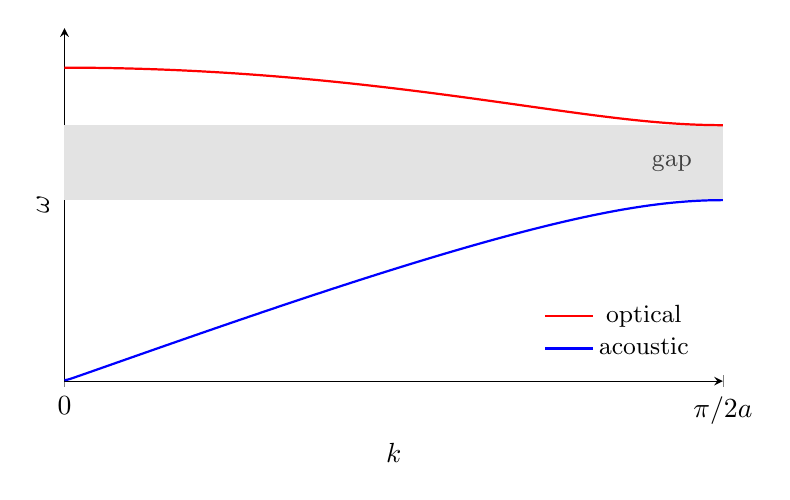
\begin{tikzpicture}
    \begin{axis}[
        width=0.82\textwidth, height=0.5\textwidth,
        xlabel={$k$}, ylabel={$\omega$},
        xmin=0, xmax=1.5708, ymin=0, ymax=1.95,
        xtick={0,1.5708}, xticklabels={$0$,$\pi/2a$},
        ytick=\empty,
        axis lines=left,
        samples=200, domain=0:1.5708,
        legend pos=south east,
        legend style={font=\small, draw=none, fill=none},
        clip=false,
    ]
    % gap band at the zone boundary (between omega_- = 1 and omega_+ = sqrt2)
    \fill[gray!22] (axis cs:0,1) rectangle (axis cs:1.5708,1.41421);
    \node[anchor=east, font=\small, gray!50!black] at (axis cs:1.52,1.2) {gap};
    \addplot[red, thick, smooth] {sqrt(1.5 + sqrt(2.25 - 2*sin(deg(x))^2))};
    \addplot[blue, thick, smooth] {sqrt(1.5 - sqrt(2.25 - 2*sin(deg(x))^2))};
    \legend{optical,acoustic}
    \end{axis}
    \end{tikzpicture}
    \caption{Acoustic (lower) and optical (upper) branches of a diatomic chain with $m_1 \neq m_2$, over half the Brillouin zone up to the boundary $k = \pi/2a$. The acoustic branch starts linearly from the origin; the optical branch has a nonzero frequency at $k = 0$. A frequency gap (shaded) separates the two branches at the zone boundary and forbids propagation at those frequencies.}
    \label{fig:diatomic}
\end{figure}
